\section{Approach}
\label{sec:appr}
In this section we present problems we identified when using unsafe plus information on how to exploit these issues in the wild.
Furthermore, we present our two tools, \toolUsage{} and \toolSA{}, that aid in locating, evaluating and fixing potentially dangerous unsafe usages in source code.

\subsection{Usage and Security Problems}
In this section, we discuss potential threat models and exploit vectors against real-world \unsafe{} Go code.

\subsubsection*{Garbage Collector Race}

\begin{itemize}
    \item Very short background on garbage collector
    \item Explain race and potential use-after-free with code pattern
    \item Explain threat model, such as information leak
\end{itemize}

\begin{figure}[!t]
    \vspace{2mm}
    \centering
    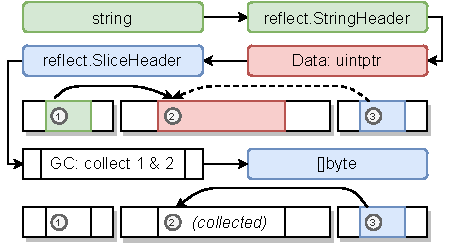
\includegraphics[width=0.4\textwidth]{gfx/figures/gcrace-vuln.pdf}
    %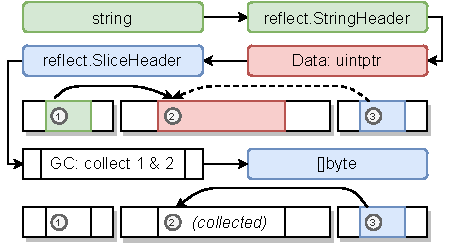
\includegraphics[width=0.48\textwidth]{gfx/figures/gcrace-vuln.pdf}
    \caption{GC race and escape analysis flaw}
    \label{fig:gcrace-vuln}
    \vspace{-8pt}
\end{figure}


Figure~\ref{fig:gcrace-vuln} shows a visualization of the casting process that leads to the problems described here.


\subsubsection*{Escape Analysis Flaw}

\begin{itemize}
    \item Very short background on escape analysis in context of Go
    \item Example code that incorrectly allocates on the stack instead of heap when using flawed cast pattern
    \item Explain threat model
\end{itemize}

\begin{lstlisting}
func main() {
	stringResult := GetString()
	fmt.Printf("main:%s\n", stringResult) // expected (but failed) stdout is "abcdefgh"
}

func GetString() string {
	b := []byte{97, 98, 99, 100, 101, 102, 103, 104}
	out := BytesToString(b)
	fmt.Printf("GetString:%s\n", out) // expected stdout is "abcdefgh"
	return out
}

func BytesToString(b []byte) string {
	bytesHeader := (*reflect.SliceHeader)(unsafe.Pointer(&b))
	strHeader := reflect.StringHeader{
		Data: bytesHeader.Data,
		Len:  bytesHeader.Len,
	}
	return *(*string)(unsafe.Pointer(&strHeader))
}
\end{lstlisting}


\subsubsection*{Implicit Read-Only}

\begin{itemize}
    \item Very short background on ELF sections and read-only property of strings
    \item Explain potential bugs (crashed) due to unnecessary complexity with in-place string casts and mutability
    \item Trade-off: performance vs. developer complexity / explicit code / potential future crashed that are hard to debug
\end{itemize}

We submitted \numberPRs{} pull requests to fix more than \numberBugsFixed{} bugs. \numberPRsMerged{} had already been accepted by the submission of this paper.


\subsection{\toolUsage{}: Automatic Identification of Unsafe Usage}

\subsubsection*{Package Identification and Unsafe Discovery}

We use the Go tool chain to identify the root module of every project, that is the module that is defined by the top-level \textit{go.mod} file in the project.

Then, we enumerate the transitive dependency packages of the project, and build the import tree. Using this import tree, we can identify the import depth as minimum depth in the tree for each package.

For each package, we then parse the code and run static code analysis on the Abstract Syntax Tree (AST). We identify usages of the following \unsafe{} tokens: \textit{unsafe.Pointer}, \textit{unsafe.Sizeof}, \textit{unsafe.Offsetof}, \textit{unsafe.Alignof}, \textit{reflect.SliceHeader}, \textit{reflect.StringHeader}, \textit{uintptr}.
We count all usages, splitting them up in the data set by their usage context as \textit{assignment}, \textit{function declaration}, \textit{call}, \textit{variable declaration}, or \textit{other}.
We save all findings including a context of some code lines for further inspection into CSV files.

\subsubsection{Architecture}

\begin{figure}[htp!]
    %\vspace{2mm}
    \centering
    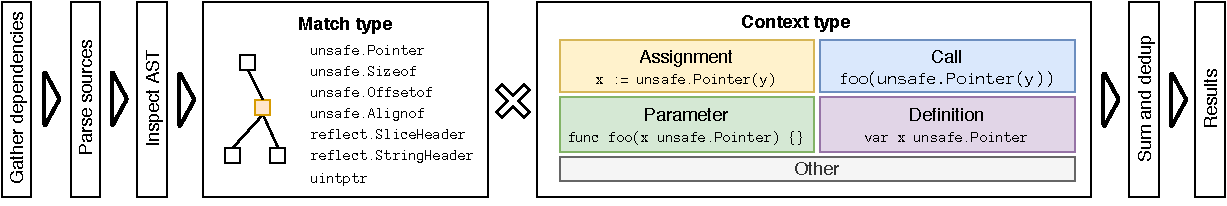
\includegraphics[width=\textwidth]{assets/figures/chapter4/go-geiger-architecture.pdf}
    \caption{Architecture of the \toolGeiger{} tool to detect unsafe usages}
    \label{fig:geiger-architecture}
    %\vspace{-10pt}
\end{figure}


Figure~\ref{fig:geiger-architecture} shows an overview of the architecture of \toolUsage{}.


\subsection{\toolSA{}: An Unsafe-focused Linter for Developers}

\subsubsection{Architecture}

Figure~\ref{fig:safer-architecture} shows an overview of the architecture of \toolSA{}.

\begin{figure}[!t]
    \vspace{2mm}
    \centering
    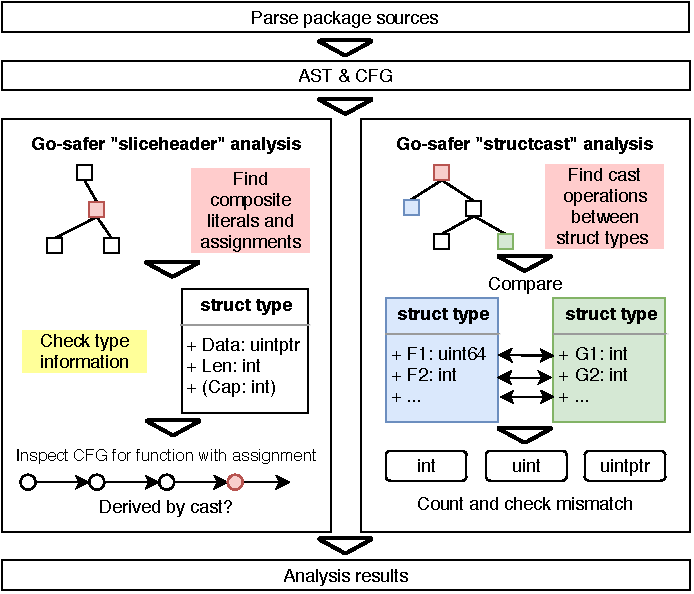
\includegraphics[width=0.48\textwidth]{gfx/figures/go-safer-architecture.pdf}
    %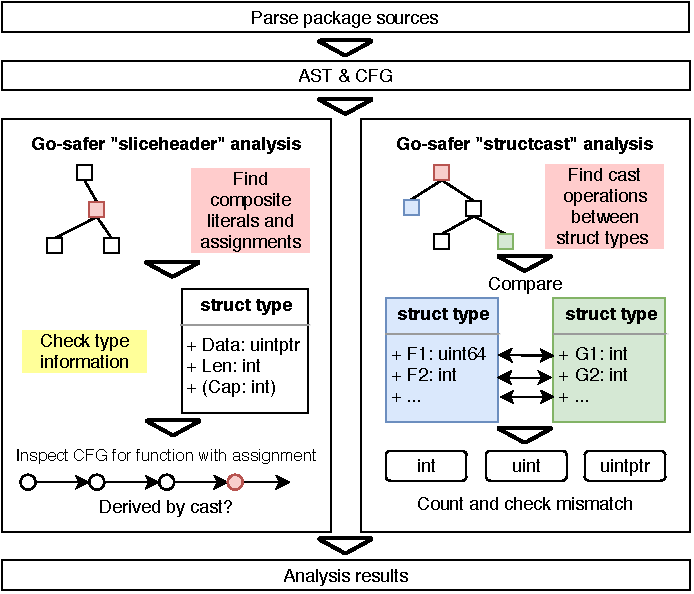
\includegraphics[width=0.45\textwidth]{gfx/figures/go-safer-architecture.pdf}
    \caption{Architecture of \toolSA{} static code analysis tool}
    \label{fig:safer-architecture}
    %\vspace{-14pt}
\end{figure}
